%\documentclass[A4,12pt]{article}
\documentclass[letterpaper,12pt]{article}
\usepackage{epsfig}
\usepackage{float}
\usepackage{amssymb,amsmath,latexsym}
\usepackage[labelformat=empty]{caption}
\usepackage{color}
%\usepackage[abs]{overpic}

\usepackage{graphicx}
\usepackage{epstopdf}

\usepackage{tikz}
\usetikzlibrary{arrows}
\usetikzlibrary{calc}
\usetikzlibrary{scopes}
\usetikzlibrary{shadows}
\usetikzlibrary{chains}
%\usetikzlibrary{shadows.blur}

\topmargin      0in 
\textheight     9.0in 
\headheight     -0.0in 
\headsep        0in
\textwidth      6.5in 
\oddsidemargin  0in 
\evensidemargin 0in
\parskip        0pt

\newcommand{\slfrac}[2]{\left.#1\middle/#2\right.}
\newcommand{\bm}    [1]{\mbox{\boldmath $#1$}}

\newtheorem{thm}           {Theorem}
\newtheorem{lemma}    [thm]{Lemma}
\newtheorem{prop}     [thm]{Proposition}
\newtheorem{property} [thm]{Property}
\newtheorem{defin}    [thm]{Definition}
\newtheorem{corollary}     {Corollary}

\begin{document}
  \noindent COM 5220 Adaptive Signal Processing \hfill 113064501  Chun-Ting Lin \\

  \begin{center}
    {\bf \large  Homework V}
  \end{center}

  %--------------------------------------------------------------
  \begin{enumerate}
    \item[{\bf 1. }]  \textbf{Adaptive Interference Canceling} \hfill \\
    Parameter specifications:
    \begin{itemize}
      \item Step size $\alpha = 10^{-2}$
      \item Maximum step size $\alpha_{\text{max}} = 10^{-2}$
      \item Minimum step size $\alpha_{\text{max}} = 10^{-4}$
    \end{itemize}
    \begin{itemize}
      \item[(a)] The learning curves of different algorithms averaging over 100 trials are 
      \begin{figure}[H]
        \centering
        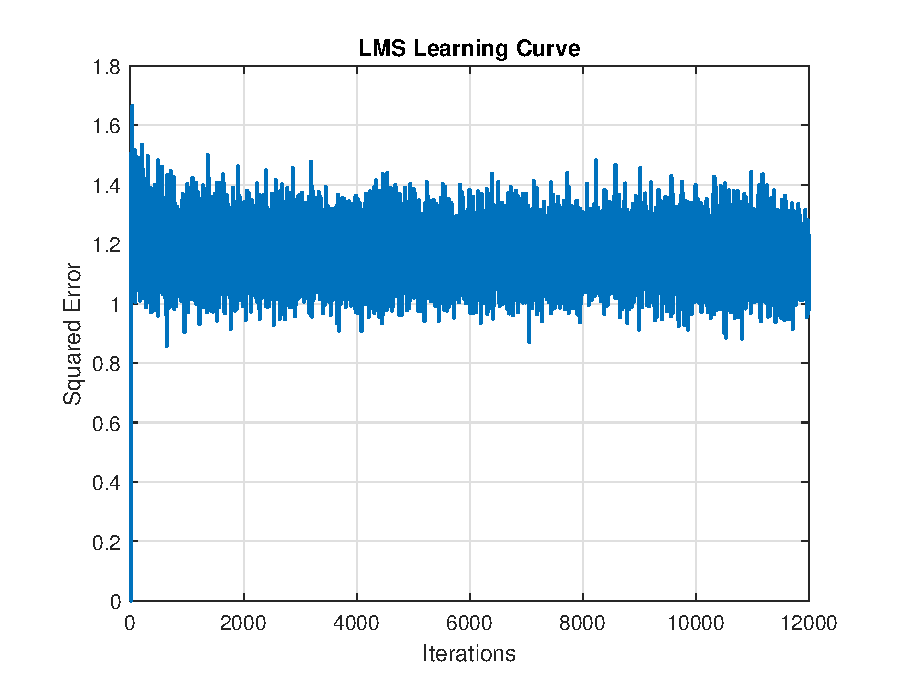
\includegraphics[scale = 0.7]{LMS.eps}
      \end{figure}
      \begin{figure}[H]
        \centering
        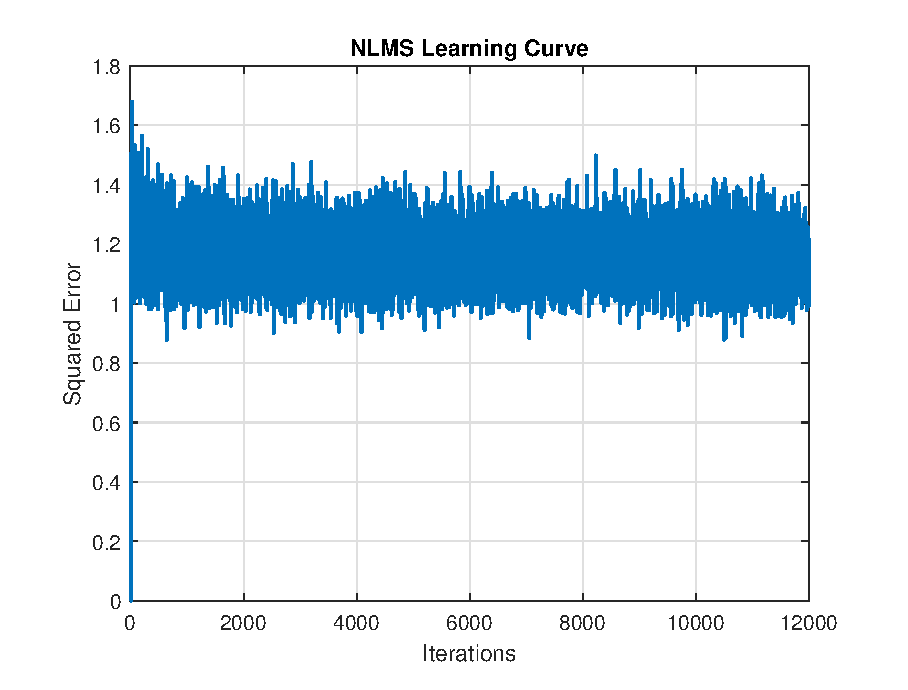
\includegraphics[scale = 0.7]{NLMS.eps}
      \end{figure}
      \begin{figure}[H]
        \centering
        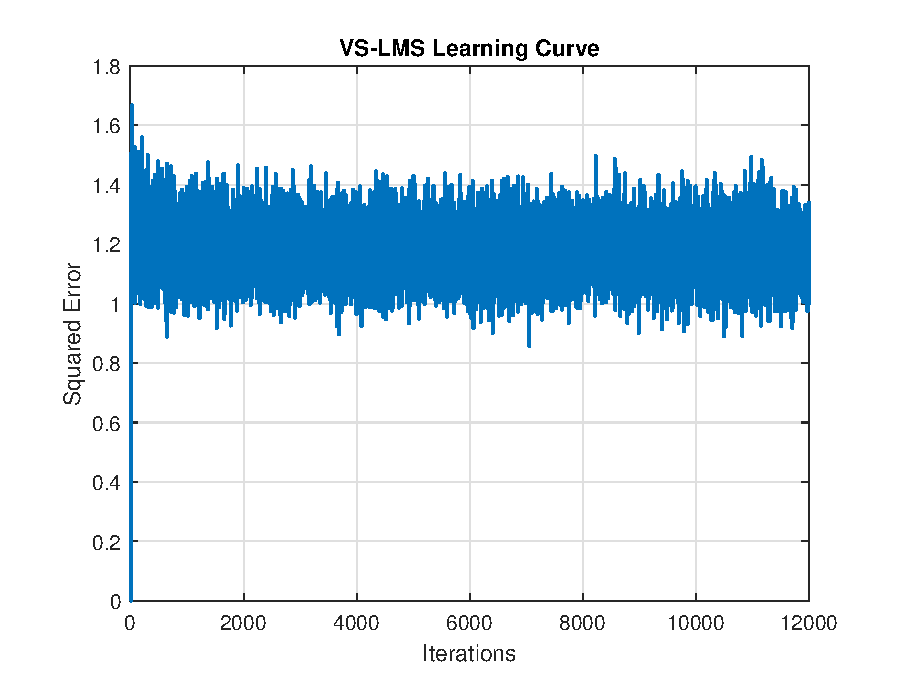
\includegraphics[scale = 0.7]{VSLMS.eps}
      \end{figure}
      \item[(b)] The BER of different algorithms averaging over 100 trials are
      \begin{table}[H]
        \centering
        \begin{tabular}{c|c|c}
                    & BER 1  & BER 2  \\
                    & (iteration = 101 $\sim$ 12000) & (iteration = 1001 $\sim$ 12000) \\
                    \hline
          LMS    & $4.06 \cdot 10^{-3}$ &  $3.94 \cdot 10^{-3}$     \\
          \hline
          NLMS   & $3.96 \cdot 10^{-3}$ &  $3.91 \cdot 10^{-3}$     \\
          \hline
          VS-LMS & $3.60 \cdot 10^{-3}$ &  $3.54 \cdot 10^{-3}$     
        \end{tabular}
      \end{table}
      \item[(C)] The average squared error of different algorithms over 100 trials are
      \begin{table}[H]
        \centering
        \begin{tabular}{c|c|c}
                    & Square Error 1                 & Square Error 2 \\
                    & (iteration = 101 $\sim$ 12000) & (iteration = 1001 $\sim$ 12000) \\
                    \hline
          LMS    & $1.69 \cdot 10^{-1}$ &  $1.67 \cdot 10^{-1}$     \\
          \hline
          NLMS   & $1.68 \cdot 10^{-1}$ &  $1.65 \cdot 10^{-1}$     \\
          \hline
          VS-LMS & $1.82 \cdot 10^{-1}$ &  $1.79 \cdot 10^{-1}$     
        \end{tabular}
      \end{table}
      \item[(d)] It is seen that the learning curves for three algorithms are vibrated near 1.3.
      If the performace metric is BER, the ranking of these thre algorithms is
      \begin{equation*}
        \text{VS-LMS} > \text{NLMS} > \text{LMS}.
      \end{equation*}
      If average squared error is chosen as performace metric, then the ranking is
      \begin{equation*}
        \text{NLMS} > \text{LMS} > \text{VS-LMS}.
      \end{equation*}
      Moreover, it can be observed that both the BER and squared error from iterations 1001 to 12000 are 
      smaller than those from iterations 101 to 12000. A possible explanation is that the algorithms have 
      not yet converged during the initial iterations.
    \end{itemize}
  \end{enumerate}
  
\end{document}
